\documentclass{book}
\usepackage[utf8]{inputenc}
\usepackage[spanish]{babel}
\usepackage{amsthm,amssymb}
\usepackage{graphicx}
\usepackage{wrapfig}
\usepackage{float}
\usepackage{tikz}
\usepackage{pgfplots}
\usepackage{lipsum}

%%%%%%%%%%%%%%%%%%%%%%%%%%%%%%%5
%\pgfplotsset{compat=1.18}
%\pgfplotsset{colormap={below}{rgb255(0cm)=(127,255,212);rgb255(1cm)=(100,149,237)}}
%\pgfplotsset{colormap={above}{rgb255(0cm)=(100,149,237);rgb255(1cm)=(65,105,225)}}

\usetikzlibrary{shapes.geometric, arrows.meta}

%%%%%%%%%%%%%%%%%%%%%%%%%%%%%%%%%%%%%%%
\title{Tutoriales de escritura en \LaTeX.}
\author{Augusto Cabrera}
\date{\today}


\decimalpoint
%%%%%%%%%%%%%%%%%%%%%%%%%%%%%%%%%%%
\begin{document}
\maketitle
%\chapter{Manejo de Gráficos.}

\section{Paquete {\bf graphicx}}

{\bf Ejemplo. Crecimiento Malthusiano}

El modelo de crecimiento de Malthus consiste en el problema de valores iniciales:

\begin{equation}
    \dot{x}(t)=\kappa x(t)
\end{equation}
con condición inicial $x(0)=X_0$.

 Tiene la solución 
\begin{equation}
    x(t)=X_0\mathrm{e}^{\kappa t}
\end{equation}

\begin{figure}[h!]
    \centering
    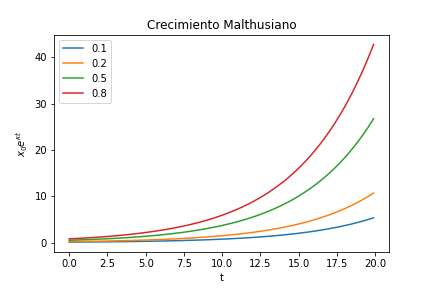
\includegraphics[scale=0.5]{malthus2.png}
    \caption{Gráfica para varias condiciones iniciales y $\kappa = 0.2$}
    \label{g2}
\end{figure}

\begin{figure}[h]
    \centering
    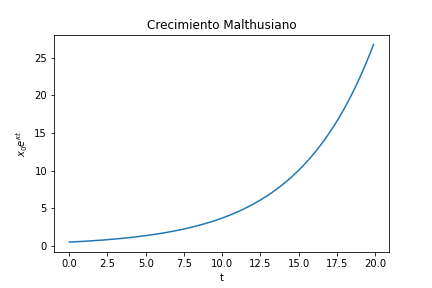
\includegraphics[scale=0.5]{malthus.png}
    \caption{Gráfica para $X_0=0.5$, $\kappa = 0.2$}
    \label{g1}
\end{figure}

 En la figura \ref{g1} podemos ver una solución para el crecimiento Malthusiano...

 \pgfplotsset{width=\textwidth,compat=1.9}

 \begin{figure}[h!]
     \centering
     \begin{tikzpicture}
         \begin{axis}[title={\bf Crecimiento Malthusiano},xlabel={\bf $t$},ylabel={\bf $X_0\rm{e}^{\kappa t}$},xmin=0,ymax=1.8]
             \addplot[color=blue]{0.5*exp(0.2*x)};
         \end{axis}
     \end{tikzpicture}
     \caption{Grafica Malthus pgfplots}
     \label{g3}
 \end{figure}

 \begin{figure}[h!]
    \centering
    \begin{tikzpicture}
\begin{axis}[title={\bf Crecimiento Malthusiano},xlabel={\bf $t$},ylabel={\bf $x_0e^{\alpha t}$}]
\addplot[color=red]{0.1*exp(0.4*x)};\addlegendentry{$x_0=0.1$}
\addplot[color=blue]{0.2*exp(0.4*x)};\addlegendentry{$x_0=0.2$}
\addplot[color=green]{0.4*exp(0.4*x)};\addlegendentry{$x_0=0.4$}
\addplot[color=purple]{0.6*exp(0.4*x)};\addlegendentry{$x_0=0.6$}
\addplot[color=black]{0.8*exp(0.4*x)};\addlegendentry{$x_0=0.8$}
\end{axis}
\end{tikzpicture}
    \caption{Gráfica para varias condiciones iniciales y $\kappa = 0.4$}
    \label{g4}
\end{figure}
%\section{Figuras con pgfplots}

Ahora dibujaremos un gráfica de una función de $\mathbb{R}$ en $\mathbb{R}$

\begin{figure}[h!]
    \centering
    \begin{tikzpicture}
        \begin{axis}
        \addplot[color=red]{exp(x)};
        \end{axis}
    \end{tikzpicture}
    \caption{Caption}
    \label{fig:enter-label}
\end{figure}

Ahora una figura en $3$-D

\begin{figure}[h!]
    \centering
    \begin{tikzpicture}
        \begin{axis}
            \addplot3[surf,]{exp(-x^2-y^2)*x};
        \end{axis}
    \end{tikzpicture}
    \caption{Caption}
    \label{fig:enter-label}
\end{figure}

\subsection{Ejemplos}

\begin{enumerate}
    \item {\bf 2D}

    \begin{figure}[h!]
        \centering
        \begin{tikzpicture}
            \begin{axis}[axis lines=left,xlabel=$x$,ylabel=$f(x)$]
             \addplot[domain=-10:10,samples=100,color=red]{x^2-2*x-1};  
             \addlegendentry{$x^2-2x-1$}

             \addplot[domain=-10:10,samples=100,color=blue]{x^2+2*x+1};
             \addlegendentry{$x^2+2x+1$}
            \end{axis}
        \end{tikzpicture}
        \caption{parábolas}
        \label{fig:enter-label}
    \end{figure}

    \item Datos

    \begin{figure}[h!]
        \centering
        \begin{tikzpicture}
            \begin{axis}
                [
                title= Dependencia de la temperatura y solubilidad del CuSO$_4$5H$_2$O,
                xlabel=Temperatura ($^{o}$C),
                ylabel=Solubilidad ($\frac{g}{100 g}$),
                xmin=0,xmax=100,
                ymin=0,ymax=120,
                xtick={0,20,40,60,80,100},
                ytick={0,20,40,60,80,100,120},
                grid style=dashed,
                ]
                \addplot[color=blue,mark=square,] coordinates {(0,23.1)(10,27.5)(20,32)(30,37.8)(40,44.6)(60,61.8)(80,83.8)(100,114)};
                \legend{CuSO$_4\cdot$5H$_2$O}
            \end{axis}
        \end{tikzpicture}
        \caption{Caption}
        \label{fig:enter-label}
    \end{figure}

    \item Barras
    \begin{figure}[h!]
        \centering
        \begin{tikzpicture}
            \begin{axis}
                [
                x tick label style={/pgf/number format/1000 sep=},
                ylabel=Años,
                enlargelimits=0.05,
                legend style={at={(0.5,-0.1)},anchor=north},
                ybar interval=0.7,             
                ]
                \addplot[color=red]coordinates{(2012,408184) (2011,408348)
		 (2010,414870) (2009,412156)};
                \addplot[color=blue] coordinates{(2012,388950) (2011,393007) 
		(2010,398449) (2009,395972)};
  \legend{Hombres, Mujeres}
            \end{axis}
        \end{tikzpicture}
        \caption{Caption}
        \label{fig:enter-label}
    \end{figure}

    \item 3D
    \begin{figure}[h!]
        \centering
        \begin{tikzpicture}
            \begin{axis}
                [
                title=Ejemplo usando mesh,
                hide axis,
                colormap/cool,
                ]
            \addplot3[mesh,samples=50,domain=-8:8,]{sin(deg(sqrt(x^2+y^2)))/sqrt(x^2+y^2)} ;
            \addlegendentry{\(\frac{sin(r)}{r}\)}
            \end{axis}
        \end{tikzpicture}
        \caption{Caption}
        \label{fig:enter-label}
    \end{figure}

    \item Contour con gnuplot
    \begin{figure}
        \centering
        \begin{tikzpicture}
\begin{axis}
[
    title={Contour plot, view from top},
    view={0}{90}
]
\addplot3[
    contour gnuplot={levels={0.8, 0.4, 0.2, -0.2}}
]
{sin(deg(sqrt(x^2+y^2)))/sqrt(x^2+y^2)};
\end{axis}
\end{tikzpicture}
        \caption{Caption}
        \label{fig:enter-label}
    \end{figure}
\end{enumerate}


%\section{Wrapfigure}

\begin{wrapfigure}{r}{0.2\textwidth}
\begin{tikzpicture}
            \begin{axis}
                [
                title=Ejemplo usando mesh,
                hide axis,
                colormap/cool, 
                width=0.5\textwidth]
            \addplot3[mesh,samples=50,domain=-8:8,]{sin(deg(sqrt(x^2+y^2)))/sqrt(x^2+y^2)} ;
            %\addlegendentry{\(\frac{sin(r)}{r}\)}
            \end{axis}
        \end{tikzpicture}
\end{wrapfigure}        
\lipsum[1-4]
\begin{wrapfigure}{l}{0.5\textwidth}
\begin{tikzpicture}
\begin{axis}
[
    title={Contour plot, view from top},
    view={0}{90}, width=0.5\textwidth
]
\addplot3[
    contour gnuplot={levels={0.8, 0.4, 0.2, -0.2}}
]
{sin(deg(sqrt(x^2+y^2)))/sqrt(x^2+y^2)};
\end{axis}
\end{tikzpicture}
\end{wrapfigure}
\lipsum[1-4]

\section{Figuras en 3D intersecadas}

\begin{figure}
    \centering
    \begin{tikzpicture}
        \begin{axis}
            [view={120}{30}]
            % parte baja del cilindro
            \addplot3[colormap/viridis,surf,z buffer=sort,samples=30,variable=\u,variable y=\v,domain=0:360,y domain=0:3]
            ({cos(u)},{sin(u)},{min(2-y,v)});
            %plano
            \addplot3[surf, z buffer= sort,samples=30,variable=\u,variable y=\v,domain=-2:2,y domain=-2:2]({u},{v},{2-v});
            %interseccion
            \addplot3[color=black,smooth,samples=30,variable=\u,domain=0:360,line width=2.5pt]
            ({cos(u)},{sin(u)},{2-sin(u)});

            %parte alta cilindro
            \addplot3[ colormap/viridis,surf,z buffer=sort,samples=30,variable=\u,variable y=\v,domain=0:360,y domain=0:4]
            ({cos(u)},{sin(u)},{max(2-y,v)});
    
        \end{axis}
    \end{tikzpicture}
    \caption{Caption}
    \label{fig:enter-label}
\end{figure}
%\begin{figure}
    \centering
    \begin{tikzpicture}
        \begin{axis}
            [
            xlabel=$x_1$,
            ylabel=$x_2$,
            zlabel=$x_3$,
            zlabel style={rotate = -90},
            xmin=-4, xmax=4,
            ymin=-5, ymax=5,
            zmin=0, zmax=2,
            ]
            \addplot3[surf, shader=faceted,samples=50,colormap/cool]{x*x-y};
            \addplot3[mesh,samples=20,color=gray](x,y,1);
            \addplot3[samples y=0,domain=-sqrt(6):sqrt(6),color=red]({x},{x*x - 1},{1});
        \end{axis}
    \end{tikzpicture}
    \caption{Caption}
    \label{fig:enter-label}
\end{figure}

\begin{figure}
    \centering
    \begin{tikzpicture}
        \begin{axis}
            [
            xlabel=$x_1$,
            ylabel=$x_2$,
            zlabel=$x_3$,
            zlabel style={rotate = -90},
            xmin=-4, xmax=4,
            ymin=-5, ymax=5,
            zmin=0, zmax=2,
            ]
            \addplot3[surf,shader=interp,samples=50,variable=\u, variable y=\v,domain=-sqrt(6):sqrt(6),y domain=0:1,colormap name=below]({u},{u*u - v},{v});
            \addplot3[mesh,samples=20,color=gray](x,y,1);
            \addplot3[mesh,samples=20,variable=\u, variable y=\v,domain=-sqrt(6):sqrt(6),y domain=1:2,colormap name=above]({u},{u*u - v},{v});
        \end{axis}  
    \end{tikzpicture}
    \caption{Caption}
    \label{fig:enter-label}
\end{figure}

\begin{figure}
    %\centering
    \begin{tikzpicture}
        \begin{axis}
            [
           z buffer=sort,data cs=polar 
            ]
            \addplot3[surf,domain=0:360,domain y=5:10, samples=30,samples y =10]{-y+5};
            \addplot3 [data cs=cart,surf,domain=-10:10, samples=2,opacity=0.25]{0};
            \addplot3[domain=0:360,samples y=0,samples=30,thick,z buffer=auto]({x},{5.1},{0});
            \addplot3[surf,domain=0:360, domain y=0:5,samples=30,samples y=10 ]{-y+5};
        \end{axis}
    \end{tikzpicture}
    \caption{Caption}
    \label{fig:enter-label}
\end{figure}

\begin{figure}
    \centering
    \begin{tikzpicture}
    \begin{axis}[domain=0.01:30]
    \addplot3[surf, opacity=0.25, blue, shader=flat] {0};
    \addplot3[surf, opacity=0.25] {(1-0.3)*e^(-x*(y/100)*(1-0.3))-e^(-x*(y/100))};
    \addplot3+[domain=4:30,samples=80,samples y=0,mark=none,black, opacity=0.5,thick]({x},{118.89/x},{0.});
\end{axis}
\end{tikzpicture}
    \caption{Caption}
    \label{fig:enter-label}
\end{figure}
\section{Diagramas con tikz}
%%%%%%%%%%%%%%%%%%%%%%%%%%%%%%%%%%%%%%%%%%%%%
\tikzstyle{startstop}=[rectangle,rounded corners, minimum width=3cm,minimum height= 1cm, text centered,draw=black, fill=red]
\tikzstyle{io}=[trapezium,trapezium left angle=70,trapezium right angle=110,minimum width=3cm,minimum height= 1cm, text centered,draw=black, fill=blue]
\tikzstyle{process}=[rectangle,minimum width=3cm,minimum height= 1cm, text centered,text width= 3cm,draw=black, fill=orange]
\tikzstyle{decision}=[diamond,minimum width=3cm,minimum height= 1cm, text centered,draw=black, fill=green]
\tikzstyle{arrow}=[thick]

%%%%%%%%%%%%%%%%%%%%%%%%%%%%%%%%%%%%%%%%%%%


\begin{tikzpicture}[node distance=2cm]
    \node (start)[startstop]{\bf Inicio};
    \node (in1)[io, below of=start]{\bf Entrada};
    \node (p1)[process, below of=in1]{\bf Proceso 1 \\ Acá empieza};
    \node (d1)[decision, below of=p1]{\bf IF};
    \node (p2a)[process,below of=d1,yshift=-1.5cm]{\bf Proceso 2 A \\ Ya casi acabamos};
     \node (p2b)[process,right of=d1,xshift=3cm]{\bf Proceso 2 B\\ Este es un proceso dummy};
    \node (o1)[io, below of=p2a]{\bf Salida};
    \node (stop)[startstop,below of=o1]{\bf Alto};
    \draw[-stealth, thick](start) -- (in1);
    \draw[-stealth, thick](in1) -- (p1);
    \draw[-stealth, thick](p1) -- (d1);
    \draw[-stealth, thick](d1) -- node[anchor=east] {\bf True} (p2a);
    \draw[-stealth, thick](d1) -- node[anchor=south] {\bf False} (p2b);
    \draw[-stealth,thick](p2b)|-(p1);
    \draw[-stealth, thick](p2a) -- (o1);
    \draw[-stealth, thick](o1) -- (stop);
\end{tikzpicture}

\end{document}
